%-----------------------------------------------------------------------------%
\chapter{\topikDua}
%-----------------------------------------------------------------------------%

%-----------------------------------------------------------------------------%
\section{Pendahuluan}
%-----------------------------------------------------------------------------%

%-----------------------------------------------------------------------------%
\subsection{Process Topologies}
%-----------------------------------------------------------------------------%

Topologi proses (\f{Process Topologies}) adalah alternatif representasi dan akses kumpulan proses paralel (\f{process group}). Tujuan dari topologi proses adalah mempermudah pembuat program dari algoritma yang menggunakan topologi seperti algoritma Cannon, Fox (\f{kartesian}) dan DNS (\f{cube})

Pada pustaka MPI, topologi proses diimplementasikan secara generik menggunakan topologi kartesian (\f{cartesian topology}) karena topologi ini sudah cukup untuk membentuk topologi lain seperti \f{line}, \f{ring}, \f{mesh}, \f{hypercube}.

Fungsi-fungsi dasar yang disediakan MPI untuk topologi kartesian adalah:
\begin{enumerate}
	\item \verb|MPI_Cart_create|: membuat topologi kartesian
	\item \verb|MPI_Cart_rank|: mendapatkan \f{rank} prosesor di topologi berdasarkan koordinat
	\item \verb|MPI_Cart_coords|: mendapatkan koordinat di topologi berdasarkan  rank
	\item \verb|MPI_Cart_shift|: mendapatkan \f{rank} tetangga (\f{neighbors}) dari sebuah prosesor
\end{enumerate}

%-----------------------------------------------------------------------------%
\subsection{Dynamic Process Generation}
%-----------------------------------------------------------------------------%

Pembuatan proses secara dinamis (\f{Dynamic Process Generation}) adalah fitur yang baru dikenalkan pada MPI v2. Fitur ini memungkinkan pembuatan proses (\f{process spawning}) secara dinamis (tidak perlu ditentukan di awal dengan opsi \verb|-n| atau \verb|-np|)

Fungsi dasar MPI untuk pembuatan proses secara dinamis

\begin{enumerate}
	\item \verb|MPI_Comm_spawn|: membuat proses secara dinamis sekaligus membuat domain komunikasi baru dengan proses tsb
	\item \verb|MPI_Comm_get_parent|: mendapatkan domain komunikasi dengan \f{parent} (pada \f{child process})
\end{enumerate}

%-----------------------------------------------------------------------------%
\section{Eksperimen}
%-----------------------------------------------------------------------------%

%-----------------------------------------------------------------------------%
\subsection{Process Topologies}
%-----------------------------------------------------------------------------%

Deskripsi program:

\begin{itemize}
	\item Kode sumber \texttt{\url{ https://github.com/yohanesgultom/parallel-programming-assignment/blob/master/problem2/demo.c}}
	\item Program ini membuat topologi cartesian 2 dimensi dengan ukuran baris ($a$) dan kolom ($b$) yang optimal untuk jumlah proses ($np$) adalah $np = a x b$ dengan fungsi \verb|MPI_Cart_create|, mencetak rank prosesor (\f{print}) topologi berdasarkan koordinat dengan \verb|MPI_Cart_rank|, mengakses prosesor berdasarkan koordinat dengan \verb|MPI_Cart_coords| dan mendapatkan tetangga (\f{neighbors}) prosesor dengan \verb|MPI_Cart_shift| 
\end{itemize}

Dengan program ini kami ingin mengamati perilaku fungsi-fungsi dasar topologi proses MPI dan mengamati waktu yang dibutuhkan untuk membuat topologi kartesian dengan variasi jumlah proses.

\begin{figure}
	\centering
	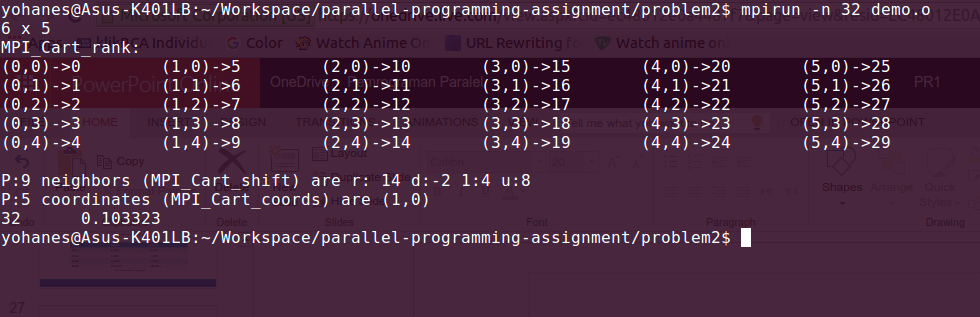
\includegraphics[width=1\textwidth]
	{pics/process_topologies_demo}
	\caption{Contoh eksekusi program demo proses topologi}
	\label{fig:process_topologies_demo}
\end{figure}  

\begin{figure}
	\centering
	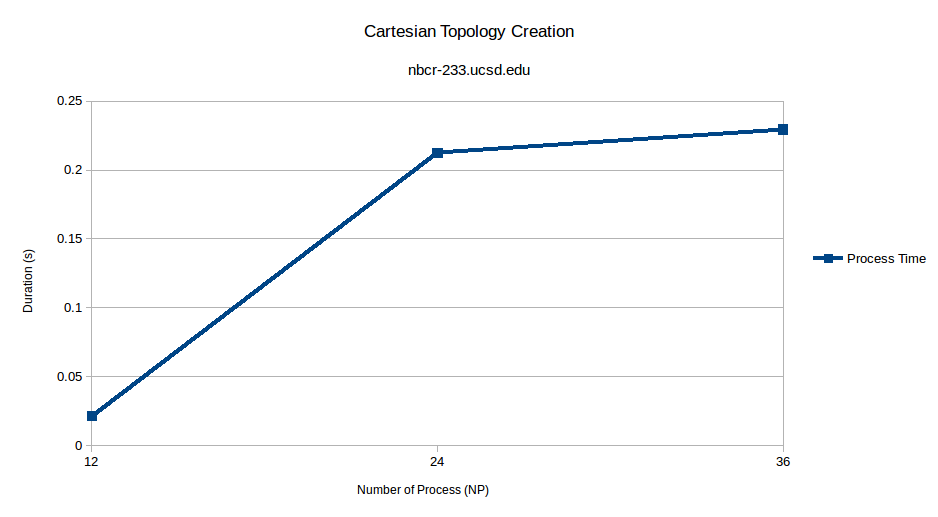
\includegraphics[width=1\textwidth]
	{pics/process_topologies_creation_nbcr}
	\caption{Eksperimen waktu pembuatan topologi kartesian di cluster UCSD}
	\label{fig:process_topologies_creation_nbcr}
\end{figure}  

Pada percobaan pertama yang hasilnya ditunjukkan pada gambar \ref{fig:process_topologies_demo}, kami mengamati bahwa fungsi \verb|MPI_Cart_shift| akan mengembalikan nilai negatif jika kita mencoba mendapatkan tetangga bawah dari proses terbawah atau tetangga teratas. Sedangkan jika kita mencoba mendapatkan tetangga kiri dari proses terkiri atau tetangga kanan dari proses terkanan, \verb|MPI_Cart_shift| akan mengembalikan \f{rank} secara \f{cyclic}.

Pada percobaan berikutnya, grafik pada gambar \ref{fig:process_topologies_creation_nbcr} menunjukkan bahwa peningkatan waktu semakin sedikit ketika topologi yang dibuat semakin besar. Dengan kata lain implementasi topologi kartesian pada MPI didesain untuk lebih optimal untuk ukuran topologi yang besar.

Program kedua yang kami gunakan adalah perkalian matriks bujursangkar dengan algoritma Cannon yang memanfaatkan topologi kartesian:

\begin{itemize}
	\item Sumber kode: \texttt{\url{https://github.com/yohanesgultom/parallel-programming-assignment/blob/master/problem2/mm_cannon.c}}
	\item Satu prosesor berlaku sebagai \manager tapi sekaligus \worker sedangkan sisanya hanya berperan sebagai \worker 
	\item Tugas \manager adalah menginisialisasi dua buah matriks bujursangkar, mempersiapkan topologi proses kartesian dengan \verb|MPI_Cart_create|, mendistribusikan pekerjaan dengan \verb|MPI_Sendrecv_replace| dan \verb|MPI_Cart_shift| untuk menentukan destinasi proses
	\item Waktu eksekusi dan komunikasi dihitung (dalam detik) menggunakan \verb|MPI_Wtime|
\end{itemize}

\begin{figure}
	\centering
	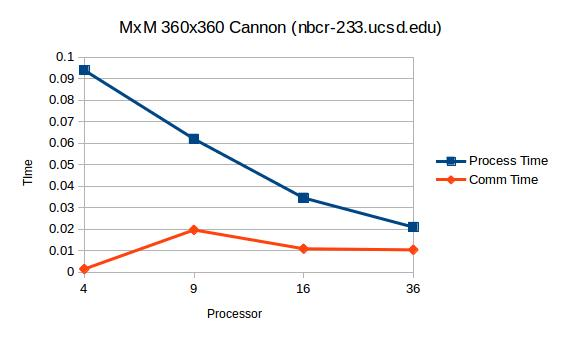
\includegraphics[width=1\textwidth]
	{pics/chart_mm_cannon_nbcr}
	\caption{Grafik hasil eksperimen algoritma Cannon cluster UCSD}
	\label{fig:result_mm_cannon_nbcr}
\end{figure}  

Percobaan ini sudah dilakukan juga pada topik sebelumnya dan hasilnya menunjukkan bahwa penggunaan topologi kartesian dapat mendukung algoritma perkalian matriks bujursangkar Cannon dalam meningkatkan efisiensi komunikasi dan memperoleh \speedup.

%-----------------------------------------------------------------------------%
\subsection{Dynamic Process Generation}
%-----------------------------------------------------------------------------%

Deskrpisi program: 
\begin{itemize}
	\item Terdapat 2 buah suprogram yaitu \manager dan \worker yang bertugas melakukan perkalian matriks-vektor dengan (\f{row-wise decomposition}). Sumber kode:
	\begin{enumerate}
		\item \texttt{\url{https://github.com/yohanesgultom/parallel-programming-assignment/blob/master/problem2/manager.c}}
		\item \texttt{\url{https://github.com/yohanesgultom/parallel-programming-assignment/blob/master/problem2/worker.c}}
	\end{enumerate}	
	\item Saat dijalankan, \manager membuat \worker sebanyak argumen yang diberikan dengan \verb|MPI_Comm_spawn|. \Worker berkomunikasi dengan manager dengan domain komunikasi yang didapat dari \verb|MPI_Comm_get_parent|. \Manager mengirimkan baris dan vektor kepada worker dengan \verb|MPI_Send| dan \verb|MPI_Bcast| untuk dikalikan secara \f{row-wise}
\end{itemize}

\begin{figure}
	\centering
	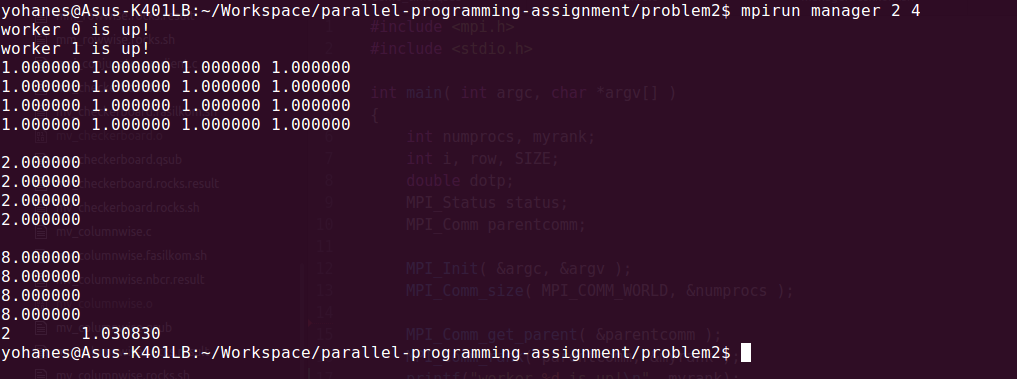
\includegraphics[width=1\textwidth]
	{pics/dynamic_process_demo}
	\caption{Contoh eksekusi program dynamic process generation}
	\label{fig:dynamic_process_demo}
\end{figure}  

\begin{figure}
	\centering
	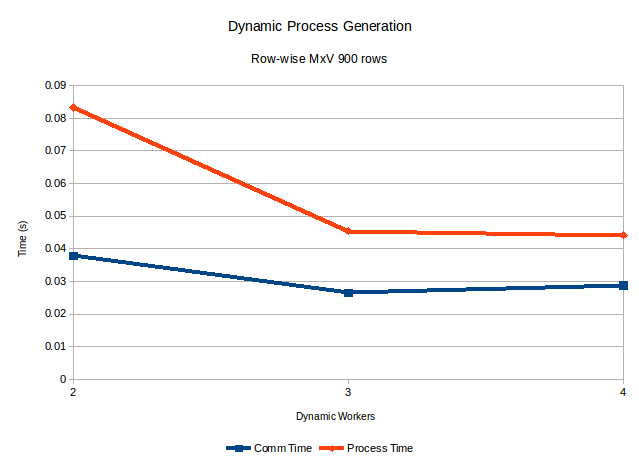
\includegraphics[width=1\textwidth]
	{pics/dynamic_process_multicore}
	\caption{Eksperimen waktu dynamic process generation di PC multicore}
	\label{fig:dynamic_process_multicore}
\end{figure}  

Pada gambar \ref{fig:dynamic_process_demo}, kami berhasil melakukan perkalian matriks-vektor dengan \f{row-wise decomposition} dengan pembuatan proses dinamis pada PC \fbox{multicore}. Sedangkan seperti yang ditunjukkan pada grafik gambar \ref{fig:dynamic_process_multicore}, perkalian matriks-vektor ini juga mengalami \speedup dari jumlah prosesor 2-4.

Selain itu, kami menemukan keterbatasan dari pembuatan proses dinamis MPI:

\begin{itemize}
	\item Tidak bisa dilakukan dengan \f{job batch/queue} (seperti di \cluster UCSD)
	\begin{itemize}
		\item Jika prosesor pada \f{job} dialokasikan sebanyak jumlah \worker maka \manager akan dibuat sebanyak jumlah \worker
		\item Jika prosesor pada \f{job} hanya dialokasikan 1, \worker gagal mendapat alokasi
	\end{itemize}
	\item Tidak bisa dilakukan pada konfigurasi cluster tertentu (\cluster Fasilkom UI)
	\item \Manager bisa melakukan \verb|MPI_Bcast| tetapi tidak bisa melakukan \verb|MPI_Send| (sepertinya terkait dengan masalah \f{ranking} pada \f{worker process group})	
\end{itemize}

%-----------------------------------------------------------------------------%
\section{Kesimpulan}
%-----------------------------------------------------------------------------%

Kesimpulan yang kami peroleh dari eksperimen ini adalah:

\begin{itemize}
	\item Fitur \f{Process Topologies} mempermudah implementasi algoritma yang membutuhkan topologi spesifik seperti algoritma Cannon
	\item \f{Dynamic Process Generation} berguna ketika sifat \f{job} dinamis (ditentukan pada saat \f{runtime}) dan/atau dibutuhkan \f{failover} (penanganan proses yang gagal)
	\item \f{Dynamic Process Generation} memiliki beberapa keterbatasan terkait spesifikasi \cluster yang digunakan. Perlu dipastikan kecocokan dengan \cluster yang akan digunakan pada saat mempertimbangkan penggunaan fitur MPI ini
\end{itemize}